\def\showsolution{1}
\documentclass[twoside]{article}
\usepackage{../quiz}

\pagestyle{myheadings}

\lstset{
    language=Python,
    basicstyle=\ttfamily,
    showstringspaces=false
    keywordstyle=\color{black},
    commentstyle=\color{black},
    stringstyle=\color{black},
    escapeinside={<*}{*>},
}

\def\semester{Fall 2016}

%%% Showing solutions %%%

\def\doshow{1}
\ifx\doshow\showsolution
\newcommand{\solution}[1]{{\color{red}#1}}
\newcommand{\solutioncircle}[1]{{\color{red}#1}}
\newcommand{\solutionimage}[2]{#2} % first arg is question, second is solution
\newcommand{\solutionblank}[2]{\hbox to #2{\color{red}#1}}
\else
\newcommand\solution[1]{} % excludes
\newcommand{\solutioncircle}[1]{#1} % don't color text but still display it
\newcommand{\solutionimage}[2]{#1} % first arg is question, second is solution
\newcommand{\solutionblank}[2]{{\rule{0pt}{2em}\underline{\hbox to #2{}}}}
\fi
\usepackage{multicol}

%%% Actual content begins here %%%
\title{\sc Discussion Quiz 7 \solution{Solutions}}

\begin{document}
\thispagestyle{empty}
\maketitle

\begin{enumerate}
%%% Q1: Scheme Primer (Conceptual) %%%
\q{1.5}{Scheme Primer (Conceptual)}

\begin{enumerate}
\item Describe all interpretations of Scheme parentheses that you can think of (in other words, say you see some parentheses... what could their meaning be?).

\solution{Parentheses either denote procedure calls or special forms. Importantly, note that every set of parentheses counts; you can never leave them out and you can never add more.}

\item On a scale from 1 to 10, where 1 is ``not at all" and 10 is ``more than anything in the world," how much do you like counting parentheses? Select one:

\begin{itemize}
\item \solution{10}
\end{itemize}

\vspace{0.02in}

\item What is a symbol in Scheme?

\solution{Symbols are like code itself -- specifically symbols are immutable, interned strings. You can think of them as variable names; in this way symbols will come in handy where interpreters are concerned!}

\end{enumerate}

%%% Q2: WWSP? %%%
\q{2}{WWSP?}

\begin{lstlisting}
scm> '((list 2 3))
<*\solution{((list 2 3))}*>

scm> (list '(2 3))
<*\solution{((2 3))}*>

scm> (define x (+))
x
scm> (define y +)
y
scm> (x 3 4)
<*\solution{Error: cannot call: 0}*>

scm> (y 3 4)
<*\solution{7}*>
\end{lstlisting}

%%% Q3: Box and Pointers %%%
\q{2.5}{Box and Pointers}

Draw box-and-pointer diagrams for each of the following Scheme lists.

\begin{lstlisting}
scm> '(2 . 3 4)
<*\solution{Error; you can only have a single element after a dot!}*>

scm> (cons (list '(two) '((3)) nil) 4)
<*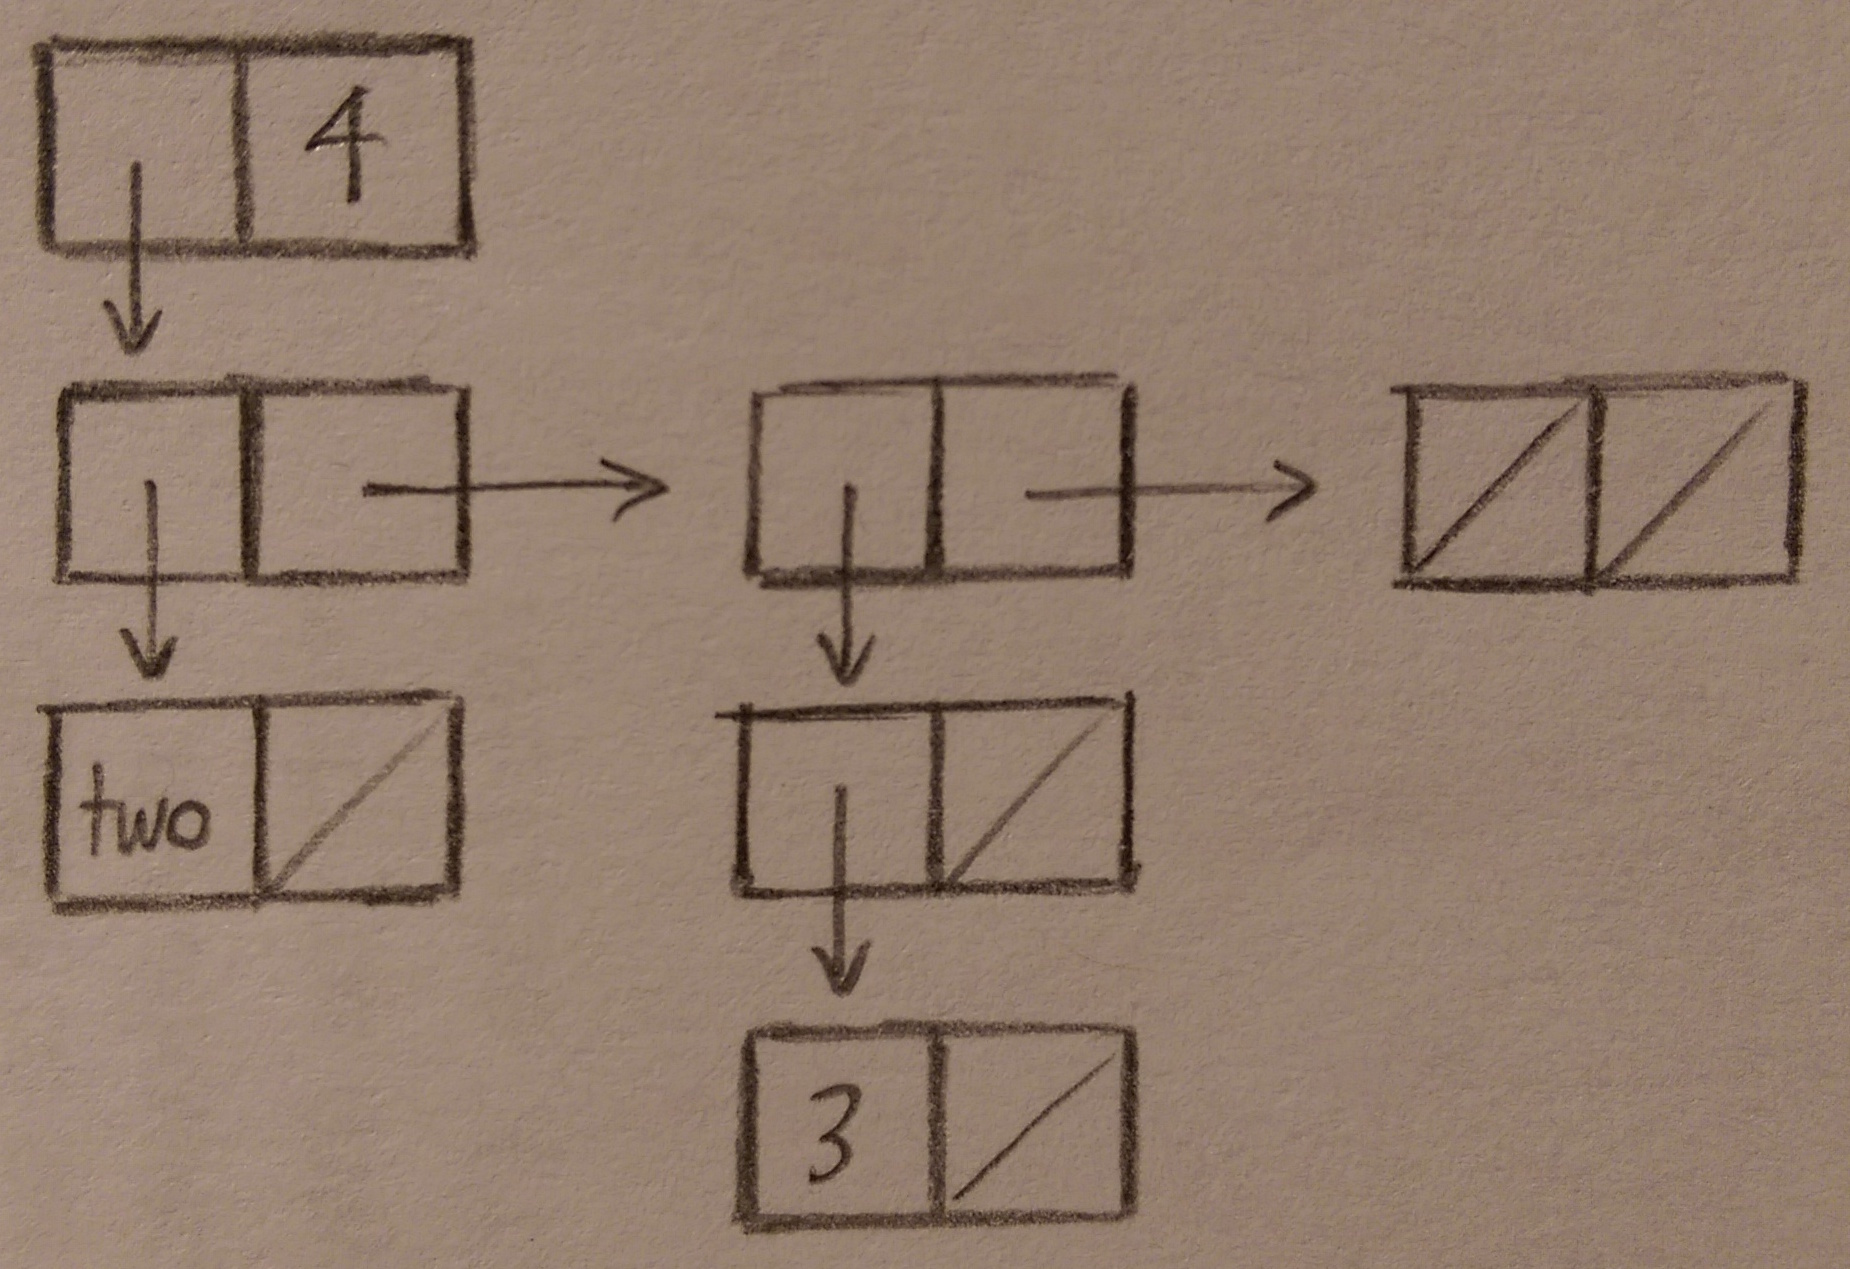
\includegraphics[scale=0.09]{2b_sol}*>

scm> (cons 2 '(list nil))
<*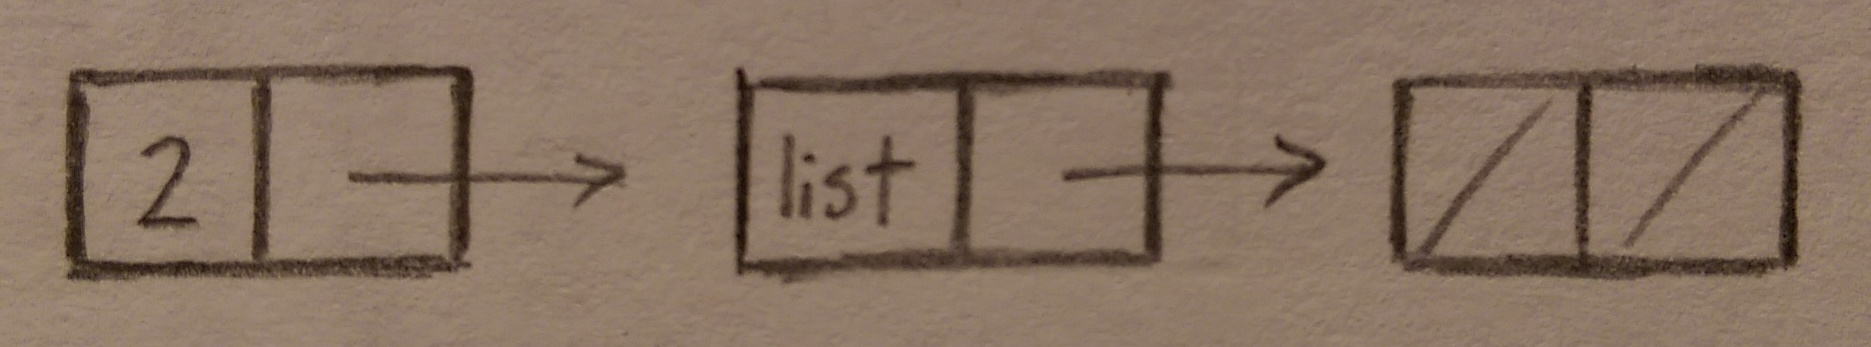
\includegraphics[scale=0.09]{2c_sol}*>

scm> (list (append '(2) '(3) nil) 4)
<*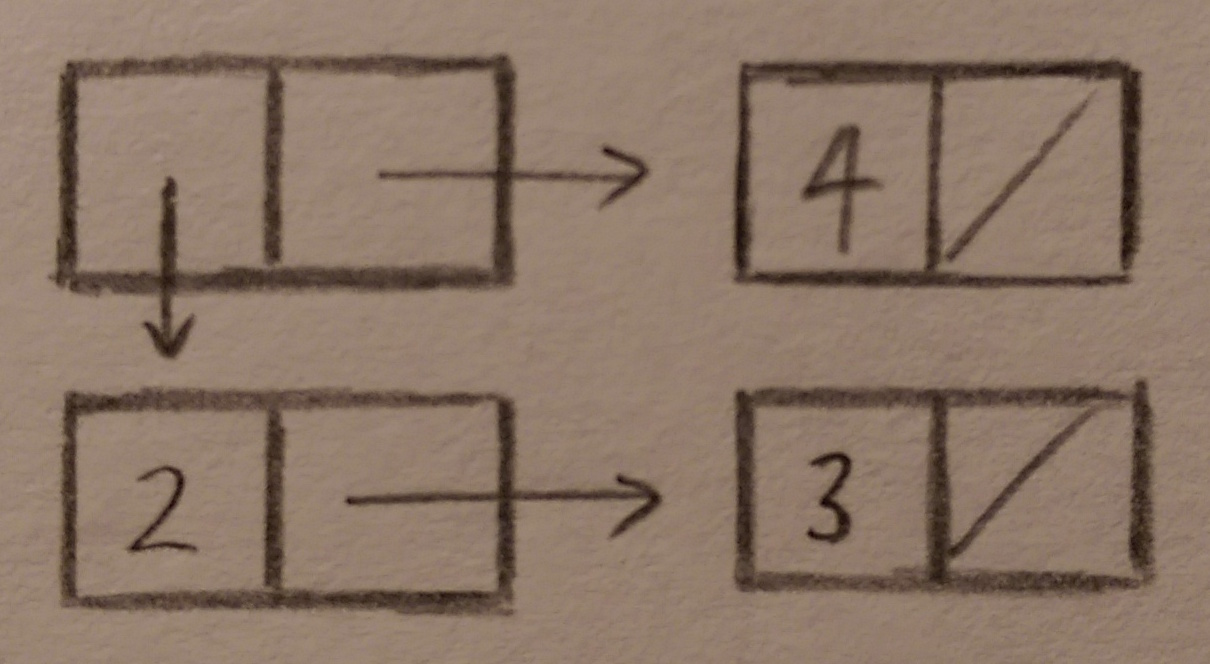
\includegraphics[scale=0.09]{2d_sol}*>

scm> '(2 . (3 . (4)))
<*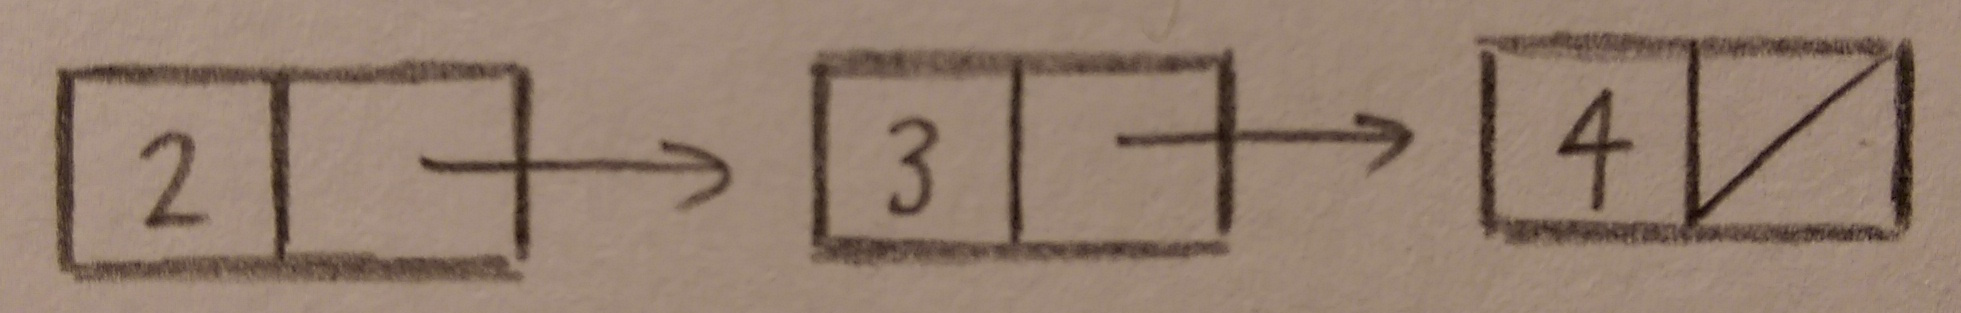
\includegraphics[scale=0.09]{2e_sol}*>
\end{lstlisting}

%%% Q4: Last One %%%
\q{4}{Last One}

Implement the procedure \texttt{finish-sort}, which takes in a well-formed list \texttt{lst} (of distinct real numbers) and returns its sorted form. You can assume that \texttt{lst} is almost sorted already, such that exactly one number is somewhere to the \textbf{right} of where it belongs and everything else is in its relatively proper place. Thus it is possible to sort the list by shifting a \textbf{single} element to the left. To balance out this relaxation, \texttt{finish-sort} is only allowed to make one pass over the data, i.e. at most one recursive call per position in the list.

\textit{Hint: you may find both the} \texttt{append} \textit{procedure and the} \texttt{let} \textit{special form helpful.}

\begin{lstlisting}
(define (finish-sort lst)
  <*\solution{(define (cadr lst) (car (cdr lst)))}*>
  <*\solution{(define (cddr lst) (cdr (cdr lst)))}*>
  <*\solution{(cond}*>
    <*\solution{((or (null? lst) (null? (cdr lst))) lst)}*>
    <*\solution{((> (car lst) (cadr lst)) (append (list (cadr lst)) (list (car lst)) (cddr lst)))}*>
    <*\solution{(else (let ((rest (finish-sort (cdr lst))))}*>
             <*\solution{(if (< (car lst) (car rest))}*>
                <*\solution{(cons (car lst) rest)}*>
                <*\solution{(append (list (car rest)) (list (car lst)) (cdr rest)))))}*>
  <*\solution{)}*>
)
\end{lstlisting}

Example usage:

\begin{lstlisting}
scm> (finish-sort '(2 3 4 5 6 7 1))
(1 2 3 4 5 6 7)
scm> (finish-sort '(2 1))
(1 2)
scm> (finish-sort '(2 9 3 11))
(2 3 9 11)
\end{lstlisting}

\end{enumerate}
\end{document}
